\documentclass{article}

% Package `amsthm` and `thmtools` must come before package `hyperref`.
\usepackage{amsthm}
\usepackage{thmtools}
% Package `hyperref` must come before package `complexity`.
\usepackage[pdftitle={Complexity of computing the size of the minimum generating set of a group}, pdfauthor={Jeffrey Finkelstein}]{hyperref}
\usepackage{complexity}
\usepackage{amsmath}
\usepackage{amssymb}
\usepackage{tikz}

\newcommand{\gen}[1]{{\langle #1 \rangle}}
\newcommand{\email}[1]{\href{mailto:#1}{\nolinkurl{#1}}}
\newcommand{\AND}{\textsc{and}}
\newcommand{\OR}{\textsc{or}}
\newcommand{\NOT}{\textsc{not}}
\newcommand{\pair}[2]{\left\langle #1, #2 \right\rangle}
\newcommand{\triple}[3]{\left\langle #1, #2, #3 \right\rangle}

\declaretheorem[numberwithin=section]{theorem}
\declaretheorem[numberlike=theorem]{conjecture}
\declaretheorem[numberlike=theorem]{lemma}
\declaretheorem[numberlike=theorem]{proposition}
\declaretheorem[numberlike=theorem, style=definition]{definition}
\declaretheorem[numberlike=theorem, style=definition]{todo}

\title{Complexity of computing the size of the minimum generating set of a group}
\author{Jef{}frey~Finkelstein}
\date{\today}

\begin{document}

\maketitle

\begin{abstract}
  \begin{abstract}
% Foreword
%
% context (focus on anyone) why now? - current situation, and why the need is so important
The rank of a finite algebraic structure with a single binary operation is the minimum number of elements needed to express every other element under the closure of the operation.
% need (focus on readers) why you? - why this is relevant to the reader, and why something needed to be done
In the case of groups, the previous best algorithm for computing rank used polylogarithmic space.
%%% relevant existing work, given as part of the need
% task (focus on author) why me? - what was undertaken to address the need
We reduce the best upper bounds on the complexity of computing rank for groups and for quasigroups. %%, and provide a theoretically efficient algorithm for the latter.
% object (focus on document) why this document - what the document covers
This paper proves that the rank problem for these algebraic structures can be verified by highly restricted models of computation given only very short certificates of correctness.

% Summary
%
% findings (focus on author) what? - what the work revealed when performing the task
Specifically, we prove that the problem of deciding whether the rank of a finite quasigroup, given as a Cayley table, is smaller than a specified number is decidable by a circuit of depth $O(\log \log n)$ augmented with $O(\log^2 n)$ nondeterministic bits (the complexity class of problems decidable by such circuits is denoted $\bFOLL$).
Furthermore, if the quasigroup is a group, then the problem is also decidable by a Turing machine using $O(\log n)$ space and $O(\log^2 n)$ bits of nondeterminism with the ability to read the nondeterministic bits multiple times (the complexity class for problems like this is denoted $\bL$).
Finally, we provide similar results for related problems on other algebraic structures and other kinds of rank.
% conclusion (focus on readers) so what? - what the findings mean for the audience
These new upper bounds are significant improvements, especially for groups.
% perspective (focus on anyone) what now? - what should be done next
In general, the lens of limited nondeterminism provides an easy way to improve many simple algorithms, like the ones presented here, and we suspect it will be especially useful for other algebraic algorithms.
\end{abstract}

\end{abstract}

\section{Introduction}

In this work we study the problem of computing the size of the minimum generating set of a group when given as a Cayley table, as well as the restriction of this problem to restricted classes of groups.
Previously, the best upper bound for this problem was $\L^2$ (also known as $\DSPACE(\log^2 n)$), due to \cite{lsz77} (also described in \cite[Proposition~3]{at06}).
The more recent work by many authors on ``bounded nondeterminism'' (in which an algorithm is allowed to nondeterministically guess a limited amount of bits and then verify the guess deterministically) as well as improved algorithms for deciding group membership due to \cite{bm89} and \cite{bklm01} allow us to improve this upper bound to $\GC(\log^2 n, \L)$ (defined in \autoref{sec:prelim}) using a more careful analysis of the original $\L^2$ algorithm.
\autoref{fig:results} summarizes the results of this work.

\begin{figure}
\caption{A summary of new upper bounds for the problem of computing the size of the minimum generating set of a group in a given class of groups.\label{fig:results}}
  \begin{center}
    \begin{tabular}{l | l}
      \multicolumn{1}{c |}{subclass $\mathcal{G}$ of \textsc{Group}}
      &
      \multicolumn{1}{| c}{upper bound for \textsc{Min Gen Size($\mathcal{G}$)}} \\
      \hline
      \hline
      \textsc{Group} & $\GC(\log^2 n, \L)$ \\
      \textsc{Nilpotent} & $\GC(\log^2 n, \L) \cap \GC(\log^2 n, \FOLL^2)$ \\
      \textsc{p-Group} & $\GC(\log^2 n, \L) \cap \GC(\log^2 n, \FOLL^2)$ \\
      \textsc{Constant Solvability Class} & $\GC(\log^2 n, \L) \cap \GC(\log^2 n, \FOLL)$ \\
      \textsc{Abelian} & $\GC(\log^2 n, \L) \cap \GC(\log^2 n, \FOLL)$ \\
      \textsc{Elementary Abelian} & $\GC(\log^2 n, \L) \cap \GC(\log^2 n, \FOLL)$
    \end{tabular}
  \end{center}
\end{figure}

The related problem of deciding group membership was placed in $\L^2$ by \cite{lsz77}, and later improved to \SL{} by \cite{bm89}.
In \cite{bklm01}, the group membership problem for several restricted classes of groups was placed in \FOLL, a class similar to $\AC^0$ but with $O(\log \log n)$ depth.
The more recent proof that $\SL = \L$ \cite{reingold08} places the membership problem for general groups (and thus for restricted classes of groups) squarely in \L.
Also related is the problem of deciding whether two given groups are isomorphic.
A series of works improved the upper bound for the \emph{quasi}group isomorphism problem (and hence the group isomorphism problem) from $\GC(\log^2 n, \P)$ \cite{py96} to $\GC(\log^2 n, \NC^2)$ \cite{wolf94} to $\GC(\log^2 n, \SAC^1)$ \cite{wagner10} to $\GC(\log^2 n, \FOLL)$ \cite{ctw10}.

\section{Preliminaries}\label{sec:prelim}

Throughout this work, $\log n$ denotes the base 2 logarithm of $n$.

\P{} is the class of decision problems decidable by a deterministic Turing machine halting in polynomial time.
$\L^2$ is the class of decision problems decidable by a deterministic Turing machine using at most $O(\log^2 n)$ space.
The (inclusion) relationship between \P{} and $\L^2$ is unknown.
\FOLL{} is the class of decision problems decidable by a $\DTIME(\log n)$-uniform family of circuits with polynomial size, unbounded fan-in, and $O(\log \log n)$ depth.
$\FOLL^2$ is the same, but with $O(\log^2 \log n)$ depth.
Following the notation of Cai and Chen \cite{cc97}, $\GC(f(n), \mathcal{C})$ is the class of decision problems decidable by a $\mathcal{C}$ machine augmented with $O(f(n))$ nondeterministic bits.
We will consider specifically the complexity classes $\GC(\log^2 n, \L)$ and $\GC(\log^2 n, \FOLL)$.

Let $P$ and $Q$ be decision problems.
We say \emph{$P$ is many-one reducible to $Q$} if there exists a function $f$ such that for all strings $x$, we have $x \in P$ if and only if $f(x) \in Q$.

A \emph{group} is a set $G$ with a binary operation $\cdot$ (the \emph{group product}) which is closed, associative, has a unique identity, and has inverses.
The \emph{product} of two elements $g$ and $h$ in $G$ is denoted $g \cdot h$, or more simply, $gh$.
A group is denoted by the pair $(G, \cdot)$, but we often just write $G$ when the group operation is clear from context or unnecessary for the current discussion.
If $T \subseteq G$, the set \emph{generated} by $T$, denoted $\gen{T}$, is the transitive closure of the group product on $T$.
We also abuse this notation and write $\gen{T_1, \dotsc, T_k , x_1, \dotsc, x_r}$ when we mean $\gen{T_1 \cup \dotsb \cup T_k \cup \{x_1, \dotsc, x_r\}}$.
A \emph{generating set} for the group $G$ is a set $T \subseteq G$ such that $\gen{T} = G$.
If $(G, \cdot)$ and $(H, \odot)$ are groups and there exists a bijective function $\phi \colon G \to H$ such that $\phi(u \cdot v) = \phi(u) \odot \phi(v)$ for all $u$ and $v$ in $G$, we say $G$ is \emph{isomorphic} to $H$ and denote this relation by $G \cong H$.

If $G$ is a finite group of order $n$, we identify the elements of the group with the indices 1, 2, \ldots, n, where 1 denotes the identity of the group.
The \emph{Cayley table} of this group is the $n \times n$ matrix with entries from $G$ in which the entry at row $u$ column $v$ has value $g$ if $u \cdot v = g$.
We consider each element of $G$ to be expressed in binary, so the size of each element is $\log n$ and thus the size of the Cayley table is $n^2 \log n$.

We will also consider subclasses of the class of all finite groups: \textsc{Group}, \textsc{Constant Solvability Class}, \textsc{Nilpotent}, \textsc{Abelian}, \textsc{p-Group}, \textsc{Elementary Abelian}, and \textsc{Cyclic}, where \textsc{Group} is the class of all finite groups, \textsc{Constant Solvability Class} is the class of all finite groups of solvability class $O(1)$, etc.
Inclusions among these classes are given in \autoref{fig:inclusions}.
\begin{figure}
  \caption{Inclusions among classes of finite groups.\label{fig:inclusions}}
  \begin{center}
    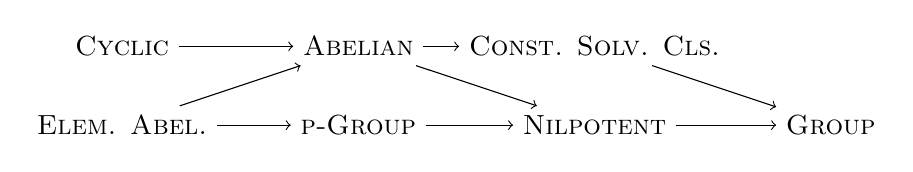
\begin{tikzpicture}[xscale=3]

      \node (e) at (0, 0) {\textsc{Elem. Abel.}};
      \node (c) at (0, 1) {\textsc{Cyclic}};
      \node (p) at (1, 0) {\textsc{p-Group}};
      \node (a) at (1, 1) {\textsc{Abelian}};
      \node (n) at (2, 0) {\textsc{Nilpotent}};
      \node (s) at (2, 1) {\textsc{Const. Solv. Cls.}};
      \node (g) at (3, 0) {\textsc{Group}};

      \path[->]
      (c) edge (a)
      (e) edge (a)
      (e) edge (p)

      (a) edge (s)
      (a) edge (n)
      (p) edge (n)

      (s) edge (g)
      (n) edge (g);
    \end{tikzpicture}
  \end{center}
\end{figure}

\section{Results}

In order to study the complexity of computing the size of the minimum generating set, we define a decision problem corresponding to this optimization problem.

\begin{definition}[\textsc{Min Gen Size($\mathcal{G}$)}]
  \mbox{}

  \textbf{Instance:} finite group $G$ (given as a Cayley table) in the class $\mathcal{G}$, natural number $k$ (given in binary).

  \textbf{Question:} Does there exist a $T \subseteq G$ such that $\gen{T} = G$ and $|T| \leq k$?
\end{definition}

Since each of the other classes of groups is a subclass of \textsc{Group}, an upper bound on the complexity of \textsc{Min Gen Size(Group)} is also an upper bound on the complexity of \textsc{Min Gen Size} for all the other subclasses.
Observe that for cyclic groups, the size of the minimum generating set is always one, so the problem is uninteresting.

\begin{theorem}
  $\textsc{Min Gen Size(Cyclic)} \in \NC^0$.
\end{theorem}

%% TODO I can't find a copy of \cite{lsz77} online.
Previously, the \textsc{Min Gen Size(Group)} problem was known to be in $\L^2$, the class of problems decidable by a deterministic Turing machine using at most $O(\log^2 n)$ space \cite{lsz77} (see \cite[Proposition~3]{at06} for a brief description of the algorithm)
We can improve this upper bound by a more careful analysis of the $\L^2$ algorithm using the following auxiliary decision problem.

\begin{definition}[\textsc{Membership($\mathcal{G}$)}]
  \mbox{}

  \textbf{Instance:} finite group $G$ (given as a Cayley table) in the class $\mathcal{G}$, finite set $S \subset G$, group element $v \in G$.

  \textbf{Question:} Is $v \in \gen{S}$?
\end{definition}

\begin{lemma}\label{lem:membershipinl}
  $\textsc{Membership(Group)} \in \L$.
\end{lemma}
\begin{proof}
  Since $\textsc{Membership(Group)} \in \SL$ \cite[Section~3]{bm89}, and $\SL = \L$ \cite{reingold08}, the lemma follows.
\end{proof}

Upper bounds on the complexity of \textsc{Membership($\mathcal{G}$)} for several subclasses of \textsc{Group} are explored in \cite{bklm01}.
%We use the logarithmic space algorithm for this problem to give a simple $\GC(\log^2 n, \L)$ algorithm for \textsc{Min Group Gen}.

Before providing the general algorithms for computing the size of the minimum generating set for classes of groups, we require one algebraic lemma which bounds the size of the minimum generating set of any finite group.

\begin{lemma}\label{lem:log}
  If $G$ is a finite group of order $n$ then the minimum size of a generating set is at most $\log n$.
\end{lemma}
%% The previous attempted proof was from
%% \url{http://math.stackexchange.com/a/226938/29369}. This proof is from
%% \url{http://www.imsc.res.in/~arvind/notes.pdf}.
\begin{proof}
  Suppose $m$ is the size of the minimum generating set.
  Let $H_0 = \gen{e}$, where $e$ is the identity element in $G$.
  For each $i \in \{1, \dotsc, m\}$, let $H_i = \gen{H_{i - 1}, x_i}$ where $x_i \in (G \setminus H_{i - 1})$.
  Such an $x_i$ must exist for each $i$ because otherwise we would have some set $H_j$, of size less than $m$, which generates the group $G$; this violates the hypothesis that $m$ is the minimum size of a generating set for $G$.

  Now, for each $i \in \{1, \dotsc, m\}$, we have $x_i \neq e$, by construction.
  Furthermore, the cosets $x_i \gen{H_{i - 1}}$ and $e \gen{H_{i - 1}}$ are disjoint.
  If we suppose to the contrary that there is some element $y \in e \gen{H_{i - 1}} \cap x_i \gen{H_{i - 1}}$, then $y = x_i h$ for some $h \in H_{i - 1}$, which implies $x_i = yh^{-1}$, and hence $x_i \in H_{i - 1}$ since both $y$ and $h$ are in $H_{i - 1}$.
  This is a contradiction with the hypothesis that $x_i \in (G \setminus H_{i - 1})$.
  Therefore $|H_i| \geq 2 |H_{i - 1}|$.
  By induction, $|G| = |H_m| \geq 2^m$, which implies $m \leq \log |G| = \log n$.
\end{proof}

This lemma allows us to consider, without loss of generality, only inputs $\pair{G}{k}$ such that $k \leq \log n$.

\begin{theorem}\label{thm:mingengc}
  $\textsc{Min Gen Size(Group)} \in \GC(\log^2 n, \L)$.
\end{theorem}
\begin{proof}
  The algorithm proceeds as follows on input $\pair{G}{k}$, where $G$ is a group of order $n$:
  \begin{enumerate}
  \item Nondeterministically guess a subset $S \subseteq G$ of cardinality at most $k$.
  \item Accept if and only if for all $v \in G$, $\triple{G}{S}{v} \in \textsc{Membership(Group)}$.
  \end{enumerate}

  First we prove that this algorithm uses $O(\log^2 n)$ nondeterministic bits and $O(\log n)$ space.
  The size of each group element, represented as number in binary, is $\log n$.
  By \autoref{lem:log}, we assume without loss of generality that the size of the minimum generating set for a group of order $n$ is at most $\log n$, so $k$ must be at most $\log n$.
  Therefore the total number of nondeterministic bits required to guess $S$ is $O(\log^2 n)$.
  Iterating over all elements of $G$ requires $O(\log n)$ space to keep track of the current element in the iteration.
  Since $\textsc{Membership(Group)} \in \L$ by \autoref{lem:membershipinl}, deciding whether $\triple{G}{S}{v} \in \textsc{Membership(Group)}$ uses at most $O(\log n)$ space.
  Therefore the total space required for this algorithm (other than the read-only input and read-only nondeterministic bits) is $O(\log n)$.

  Next we show that the algorithm correctly decides the problem.
  Suppose $\pair{G}{k} \in \textsc{Min Gen Size(Group)}$, so there exists a $T \subseteq G$ such that $|T| \leq k$ and $\gen{T} = G$.
  One of the sets $S$ of cardinality at most $k$ that the algorithm guesses will equal $T$, since $|T| \leq k$.
  For all elements $v \in G$, we have $v \in \gen{T}$ since $\gen{T} = G$.
  Hence the (correct) algorithm for \textsc{Membership(Group)} will accept for all $v \in G$, and the overall algorithm will accept.
  For the converse, suppose the algorithm accepts the input $\pair{G}{k}$.
  This occurs exactly when it has guessed a set $S$ of cardinality at most $k$ such that all elements $v$ in $G$ are members of the subgroup generated by $S$.
  Thus $S$ is a generating set for $G$ of cardinality at most $k$, so $\pair{G}{k} \in \textsc{Min Gen Size(Group)}$.
\end{proof}

This improves the previous upper bound, $\L^2$, for general groups because
\begin{equation*}
  \GC(\log^2 n, \L) \subseteq (\NL \cap \GC(\log^2 n, \NC^2)) \subseteq (\NL \cup \GC(\log^2 n, \NC^2)) \subseteq \L^2.
\end{equation*}
(In the first inclusion we use the fact that $\L \subseteq \NL \subseteq \NC^2$.
In the last inclusion we use Savitch's Theorem and the fact that $\GC(\log^d n, \NC^k) \subseteq \L^{\max{(d, k)}}$ \cite[Lemma~3.1]{wolf94}.)
This also immediately improves the result of \cite[Theorem~7]{at06}, which shows \textsc{Min Gen Size(Nilpotent)} is in \P, since
\begin{equation*}
  \GC(\log^2 n, \L) \subseteq \NL \subseteq \P.
\end{equation*}
We can provide further upper bounds by using the fact that restricted classes of groups have more efficient algorithms for deciding subgroup membership.

\begin{theorem}
  \mbox{}
  \begin{enumerate}
  \item Each of the problems
    \begin{itemize}
    \item \textsc{Min Gen Size(Constant Solvability Class)},
    \item \textsc{Min Gen Size(Abelian)},
    \item \textsc{Min Gen Size(Elementary Abelian)}, and
    \item \textsc{Min Gen Size(Cyclic)}
    \end{itemize}
    is in $\GC(\log^2 n, \FOLL)$.
  \item Each of the problems
    \begin{itemize}
    \item \textsc{Min Gen Size(Nilpotent)} and
    \item \textsc{Min Gen Size($p$-Group)}
    \end{itemize}
    is in $\GC(\log^2 n, \FOLL^2)$.
  \end{enumerate}
\end{theorem}
\begin{proof}
  \mbox{}
  \begin{enumerate}
  \item
    We know that the membership problem for each of these classes of groups is in \FOLL{} by \cite[Section~3]{bklm01}.
    A slight modification of the algorithm from \autoref{thm:mingengc} can be used to show that each of these problems is in $\GC(\log^2 n, \FOLL)$.
    After nondeterministically guessing a set $S$, instead of iterating over each element of the group in logarithmic space, we use in parallel $n$ instances of the \FOLL{} circuit which decides the membership problem and compute the conjunction of the output of each of the instances for one additional layer of depth and a $O(n)$ increase in the size of the circuit.
    Since the size of the circuit remains polynomial in $n$ and the depth remains $O(\log \log n)$, we have shown that the problem is in $\GC(\log^2 n, \FOLL)$.
  \item
    The same argument applies, except using the fact that the membership problem for nilpotent groups is in $\FOLL^2$ \cite[Corollary~3.12]{bklm01}.
    Also, every finite $p$-group is nilpotent. \qedhere
  \end{enumerate}
\end{proof}

We can now show some negative completeness results, providing more specific upper bounds for the complexity of computing the size of the minimum generating set of a group.
Although, the precise relationship between \FOLL{} (and between $\FOLL^2$) and \L{} is unknown, \FOLL{} does not contain any class containing the \textsc{Parity} problem.
Since \textsc{Parity} is in \L, we know \FOLL{} does not contain \L.
Stated in a slightly more general way, neither \FOLL{} nor $\FOLL^2$ can be hard under $\AC^0$ many-one reductions for any complexity class that contains \textsc{Parity} \cite[Proposition~2.1]{bklm01}.
This is true even when the circuit is augmented with a polylogarithmic number of nondeterministic gates \cite[Section~4]{ctw10}.
This gives an immediate improvement to the upper bound of all the problems shown in the previous section to be in $\GC(\log^2 n, \FOLL^2)$.

\begin{theorem}
  None of the decision problems
  \begin{itemize}
  \item \textsc{Min Gen Size(Nilpotent)},
  \item \textsc{Min Gen Size(p-Group)},
  \item \textsc{Min Gen Size(Constant Solvability Class)},
  \item \textsc{Min Gen Size(Abelian)},
  \item \textsc{Min Gen Size(Elementary Abelian)}, or
  \item \textsc{Min Gen Size(Cyclic)}
  \end{itemize}
  are hard under $\AC^0$ many-one reductions for any complexity class containing \textsc{Parity}, specifically those in the inclusion chain
  \begin{equation*}
    \ACC^0 \subseteq \TC^0 \subseteq \NC^1 \subseteq \L \subseteq \NL \subseteq (\LOGCFL \cup \DET).
  \end{equation*}
\end{theorem}

\section{Future work}

As noted in the introduction, the (quasi)group isomorphism problem is known to be in $\GC(\log^2 n, \FOLL)$.
What is the relationship between this problem and the minimum generating set size problem for groups?

What is the precise relationship between computing the minimum generating set and computing the size of the minimum generating set?
An efficient function which computes the minimum generating set implies an efficient function which computes the size of the minimum generating set (compute the set, then compute its cardinality), so we know that the former must be at least as hard as the latter.
On the other hand, it seems unlikely that knowing the size of a minimum generating set would yield any information about the contents of such a set.

\section{About this work}

Copyright 2013 Jef{}frey Finkelstein.

This work is licensed under the Creative Commons Attribution-ShareAlike License 3.0.
Visit \mbox{\url{https://creativecommons.org/licenses/by-sa/3.0/}} to view a copy of this license.

The \LaTeX{} markup which generated this document is available on the World Wide Web at \mbox{\url{https://github.com/jfinkels/mingroupgen}}.
It is also licensed under the Creative Commons Attribution-ShareAlike License.

The author can be contacted via email at \email{jeffreyf@bu.edu}.

\bibliographystyle{plain}
\bibliography{references}

\end{document}
